\graphicspath{{Kapitel/Kapitel4_Hauptteil/Images/}}

Dieses Kapitel beschreibt die Virtual Reality Applikation \textit{C.LABEL-VR} und ist somit der Hauptteil dieser Arbeit. Das Ziel dieser Applikation ist es die Annotierung von Punktwolken, wie sie beispielsweise in C.LABEL möglich ist, innerhalb einer dreidimensionalen Umgebung zu realisieren. Dazu müssen zunächst Datenformate eingelesen werden, die Informationen über Punktwolken enthalten. Anschließend müssen aus diesen Daten Punktwolken erzeugt werden. Der Vorgang des Imports wird in Kapitel \ref{sec:ImportExport} näher beschrieben, die Erzeugung der Punktwolken in \ref{sec:Generierung}. Um sich in der virtuellen Umgebung durch diese Wolken bewegen zu können, wurden diverse Möglichkeiten zur Navigation entwickelt. Auf die Funktion dieser Möglichkeiten und deren Auswirkungen auf das Befinden des Menschen (\textit{Virtual Motion Sickness}) wird in Abschnitt \ref{sec:Navigation} eingegangen.\\

Anschließend geht es um die Annotierung der generierten Punktwolken. Annotierung bedeutet in diesem Kontext, dass die einzelnen Punkte der Wolken mit bestimmten Klassifikationen versehen werden, welche der Art des Objektes entsprechen, dem die Punkte zugehören. Ist der Punkt beispielsweise Bestandteil eines Autos, so wird er mit der Klasse \textit{Auto} versehen. Um diese Aufgabe erfüllen zu können wurden mehrere Arten der Annotierung entwickelt. Welche dies sind und wie sie realisiert wurden, wird in Abschnitt \ref{sec:Annotation} gezeigt. Das letzte Kapitel \ref{sec:UIMenu} beschäftigt sich mit der Benutzerschnittstelle der Applikation. Dieses wird auch \textit{User Interface} oder kurz \textit{\acrshort{acr:UI}} genannt. Dabei wird hauptsächlich auf die Funktionen des Menüs eingegangen welches man während des Labelns aufrufen kann. Ebenfalls wird erläutert welche Herausforderungen es bei der Erstellung von \acrshort{acr:UI}s in der virtuellen Realität gibt und wie diese bewältigt wurden. Zur Veranschaulichung aller Funktionen von C.LABEL-VR ist in der Abbildung \ref{fig:Workflow} der grobe \gls{glos:Workflow} in Form eines Diagramms abgebildet.

\begin{figure}%
	\centering
    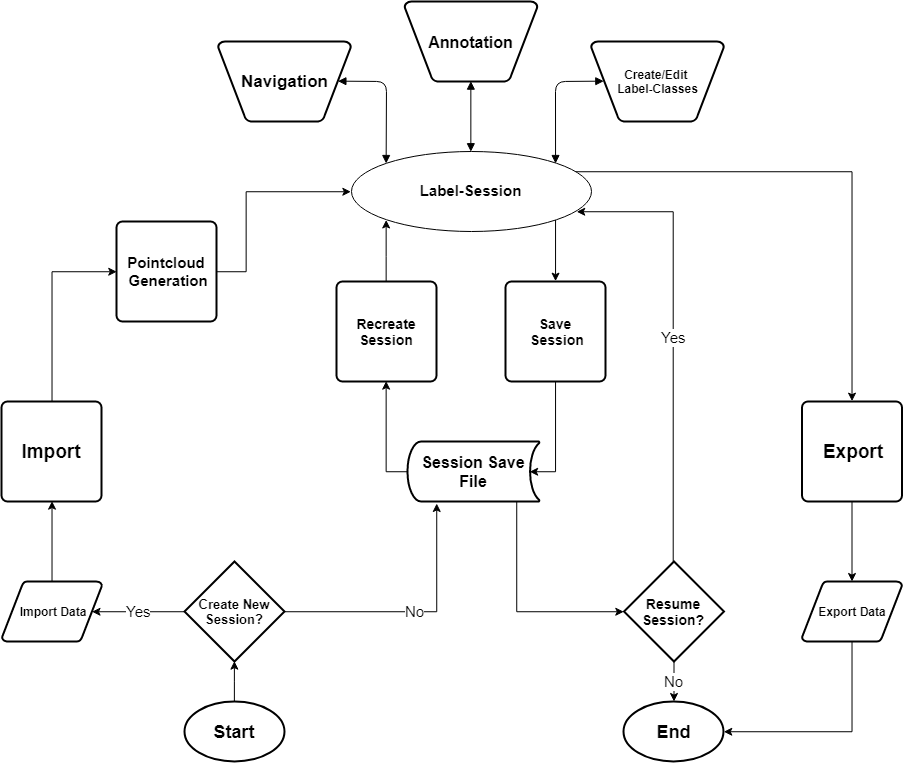
\includegraphics[width=13.5cm]{Workflow}
    \caption{\glslink{glos:Workflow} in C.LABEL-VR vom Import bis zum Export}
    \label{fig:Workflow}
\end{figure}

\section{Import und Export von Daten}
\label{sec:ImportExport}
Umfeldmodelle, welche in Form einer Punktwolke vorliegen, werden meist von einem Radar-, oder, wie in Kapitel \ref{sec:Lidar} gezeigt, von einem Lidar-Sensor aufgenommen. Die Informationen über diese Modelle, zum Beispiel die Positionen der einzelnen Punkte, werden in einem passenden Datenformat abgespeichert. Um welches Format es sich dabei handelt kann sehr unterschiedlich sein. In der Regel hängt es davon ab zu welchem Zweck die aufgenommenen Daten gebraucht werden und wie umfangreich diese Daten sind. Am häufigsten werden sie dafür verwendet um Lernalgorithmen und neuronale Netze (siehe Abschnitt \ref{sec:KNN}) zu trainieren. Automobilhersteller haben für solche Vorhaben natürlich unterschiedliche Konzepte und somit können auch die Formate der Daten unterschiedlich sein. Um die Applikation \textbf{C.LABEL-VR} für mehrere dieser Hersteller benutzbar zu machen, muss das Programm also mit verschiedenen Datenformaten umgehen können.\\ 

Innerhalb dieser Arbeit wurden mit zwei verschiedenen Arten von Daten gearbeitet. Das erste Format ist das PCD-Format (\textit{Point Cloud Data}). Die Bibliothek PCL(\textit{Point Cloud Library}) benutzt das Datenformat \textbf{PCD} um Informationen über Punktwolken zu verwalten. PCL ist eine sehr mächtige C++-Bibliothek, die in der Regel von jedem benutzt wird, der performante Algorithmen für Punktwolken entwickeln möchte. Auch C.LABEL generiert aus eingelesenen Daten PCD-Files um Funktionen der Point Cloud Library für die Wolken zu benutzen.\\

Das zweite Format ist das, von der HDF-Group bereitgestellte, HDF5-Format (\textit{Heterogeneous Data Format}). Es ist ausgelegt zum schnellen Erstellen und Auslesen von komplexen und großen Datenstrukturen. Welche Elemente diese Strukturen enthalten können wird später in Kapitel \ref{sec:HDF5} erklärt. Zur schnellen Bearbeitung großer Datenmengen ist dies ein gängiges Format und wird von den meisten Kunden von CMORE benutzt um Sensordaten zu verwalten. Deshalb wird es auch in C.LABEL-VR verwendet.\\

\subsection{Architektur}

Wichtig ist es also sowohl den Import, als auch den Export so modular wie möglich zu gestalten, dass C.LABEL-VR ohne große Änderungen  an der Hauptapplikation um neue Datenformate erweitert werden kann. Das Prinzip, das dafür entwickelt wurde, ist in Abbildung \ref{fig:ImportExport} dargestellt und wird im Folgenden näher erläutert. Die angesprochenen Erweiterungen um neue Datenformate werden als \textit{Addons} bezeichnet. Jedoch handelt es sich dabei nicht immer nur um eine Erweiterung eines, von Grund auf, neuen Datenformates. 
Bei Komplexen Datenformaten wie HDF5 kann der Entwickler die interne Struktur der Datei selbst bestimmen. Jede unterschiedliche Struktur muss auf unterschiedliche Weise eingelesen werden und braucht somit unterschiedliche Addons. Um die Erweiterbarkeit der Applikation sicherzustellen wurde der Import und der Export von der Hauptapplikation abgekapselt.

Dafür wurde eine interne Datenstruktur (kurz \acrshort{acr:IDS}) eingeführt, welche alle nötigen Informationen enthält, die für das \glslink{glos:Labeling}{Labeling} notwendig sind. Sie wird im späteren Kapitel \ref{sec:IDS} genauer vorgestellt. Der Vorteil dabei ist, dass die Hauptapplikation dadurch stets auf die gleiche Datenstruktur zurückgreifen kann. Sie bleibt somit unabhängig vom importierten Datenformat. Wird ein neues Import-Format eingeführt muss an der Hauptapplikation also nichts verändert werden. In der Abbildung \ref{fig:ImportExport} erkennt man, wie die Hauptapplikation (\textit{C.LABEL-VR Session}) nur mit internen Daten arbeitet und somit von den Import- und Exportdaten getrennt ist.\\ 

Jedes Import-Addon hat also zunächst die Aufgabe, seine jeweiligen Daten einzulesen und alle Informationen, die für die \acrshort{acr:IDS} notwendig sind, daraus zu extrahieren. Aus diesen Informationen können anschließend die entsprechenden Punktwolken generiert werden. Die Generierung wird in Kapitel \ref{sec:PclGenerate} erklärt. Beim Export ist es notwendig, dass die Struktur der Daten gleich bleibt, die vom Import-Addon eingelesenen wurden. Es sollen lediglich die \glslink{glos:Labeling}{Labeling}-Informationen aus der \acrshort{acr:IDS} hinzu- bzw. eingefügt werden. Aus der \acrshort{acr:IDS} kann das Export-Addon diese Informationen extrahieren und anschließend in die eingelesenen Daten exportieren. Die importierten Daten werden so allerdings überschrieben. Möchte man die Daten nicht überschreiben, müssen die Daten neu erstellt und mit den \glslink{glos:Labeling}{Labeling}-Informationen versehen werden. \\

Die Importierten Daten, beispielsweise HDF5, enthalten allerdings oft deutlich mehr Informationen, als für die interne Struktur notwendig. Diese Zusatzinformationen werden \textit{Metadaten} genannt. Für den Export bedeutet dies, dass man aus der internen Datenstruktur von C.LABEL-VR, die Struktur der anfangs eingelesenen Daten nicht wieder rekonstruieren kann, da die \textit{Metadaten} fehlen würden. Um dieses Problem zu lösen müssen die zusätzlichen Daten separat gespeichert werden. Dazu wurde eine erweiterbare Datenstruktur angelegt. In dieser kann man für jede Import-Struktur eine Metadatenstruktur anlegen. Das entsprechende Export-Addon kann die Metadaten dann verwenden um, zusammen mit den internen Daten, das gewünschte Exportformat zu rekonstruieren. \\

\begin{figure}%
	\centering
    \includegraphics[width=13.5cm]{Import_Export_Architecture}
    \caption{Das Import-Export-Prinzip in C.LABEL-VR}
    \label{fig:ImportExport}
\end{figure}

Zusammenfassend ist also folgendes zu tun, um die Benutzung ein neues Datenformates oder einer neuen Datenstruktur zu gewährleisten: Zunächst muss eine Importfunktion programmiert werden, die alle Informationen aus den gewünschten Daten ausliest. Anschließend muss diese Funktion das genormte, interne Datenformat (Kapitel \ref{sec:IDS}) erstellen und alle nötigen Informationen aus den eingelesenen Daten darin speichern.  Daraus können die entsprechenden Punktwolken dann generiert werden können. Falls es Daten gibt, die über diejenigen in der \acrshort{acr:IDS} hinausgehen, muss eine Metadatenstruktur angelegt werden, in welche die zusätzlichen Daten abgelegt werden können. Zuletzt ist eine Exportfunktion zu implementieren, welche die \glslink{glos:Labeling}{Labeling}-Informationen aus der internen Datenstruktur in die eingelesenen Daten exportieren kann. Außerdem muss sie in der Lage sein aus den internen- und den Metadaten das Ausgangsdatenformat wiederherzustellen, um die Daten als neue Files exportieren zu können. Im folgenden Kapitel soll dieses Prinzip konkret an einem HDF5-Beispiel gezeigt werden.

\subsection{HDF5-Beispiel}
\subsubsection{HDF5 Daten}
\label{sec:HDF5}
\subsubsection{Beispiel}

\section{Generierung einer Punktwolke}
\label{sec:Generierung}

\subsection{Interne Datenstruktur}
\label{sec:IDS}

\subsection{Generierung}
\label{sec:PclGenerate}
%session
%pointcloud
%...

%Koordinatensysteme

\subsection{Optimierung}
TODO
Methoden zur FPS-Steigerung

%-generell nichts teures in update mehthode
%	
%-gameobject find
%-getcomponent
%
%keine update oder start mehtode bei skripten der punkte
%collider trigger nicht bei den punkten sondern beim anderen object
%generell alle pollenden aktionen von den punkten entfernen
%
%
%(-clonen von prefabs statt neue instanzen von inbuilts)
%shared materials verwenden   kein material.color weil das eine kopie des materials erzeugt, welches dann einzeln gecallt werden muss
%
%gpu instancing bei den materials verwenden und forward rendering options

\section{Navigation}
\label{sec:Navigation}
\subsection{VR-Krankheit}
\subsection{Freier Flug}
\subsection{Teleport}

\section{Annotieren der Punktwolke}
\label{sec:Annotation}
\subsection{Einfache Pointer Annotation}
\label{sec:SimplePointerAnnotation}

\subsection{Cluster Annotation}
In einer Punktwolke mit mehreren tausend Punkten wird es für den Benutzer auf Dauer mühsam jeden Punkt einzeln zu Annotieren. Bei diesem Problem soll die \textit{Cluster Annotation} Abhilfe schaffen. Diese Art der Annotation soll selbstständig die Punkte in einen Cluster aufnehmen und sie mit der gleichen Klasse labeln, die zum gleichen Objekt gehören. Der Benutzer wählt hierfür, wie im vorherigen Kapitel \ref{sec:SimplePointerAnnotation} einen Punkt mit Hilfe des Pointers aus. Ausgehend davon werden umliegende Punkte untersucht, ob sie zum gleichen Objekt gehören wie der ausgewählte Startpunkt. Ist dies der Fall werden sie in den Cluster aufgenommen. Werden keine Punkte mehr aufgenommen bleibt der Endcluster übrig, welcher dann einem Objekt entspricht, zum Beispiel einem Auto. \\

Wissenschaftler beschäftigen sich intensiv mit solchen Verfahren zur Objektidentifizierung in dreidimensionalen Punktwolken. Ansätze, wie sie in \cite{bib:Segmentation1}, \cite{bib:Segmentation2} oder \cite{bib:Segmentation3} vorgestellt werden sind nur wenige von vielen. Die meisten haben aber ein ähnliches Vorgehen. Zuerst werden all diejenigen Punkte in der Wolke entfernt, die zum Boden gehören. So bleiben anschließend nur noch Punkte übrig, welche zu Objekten wie beispielsweise Autos, Häuser oder Straßenschilder gehören. Die übrig gebliebenen Punkte können nun mit diversen Algorithmen zu Clustern zusammengefasst werden. Ein Beispiel für das Ergebnis eines solchen Verfahrens bietet die Abbildung \ref{fig:ClusteredCloud}. Im Folgenden wird vorgestellt wie die Cluster-Analyse in C.LABEL-VR funktioniert.

\begin{figure}%
	\centering
    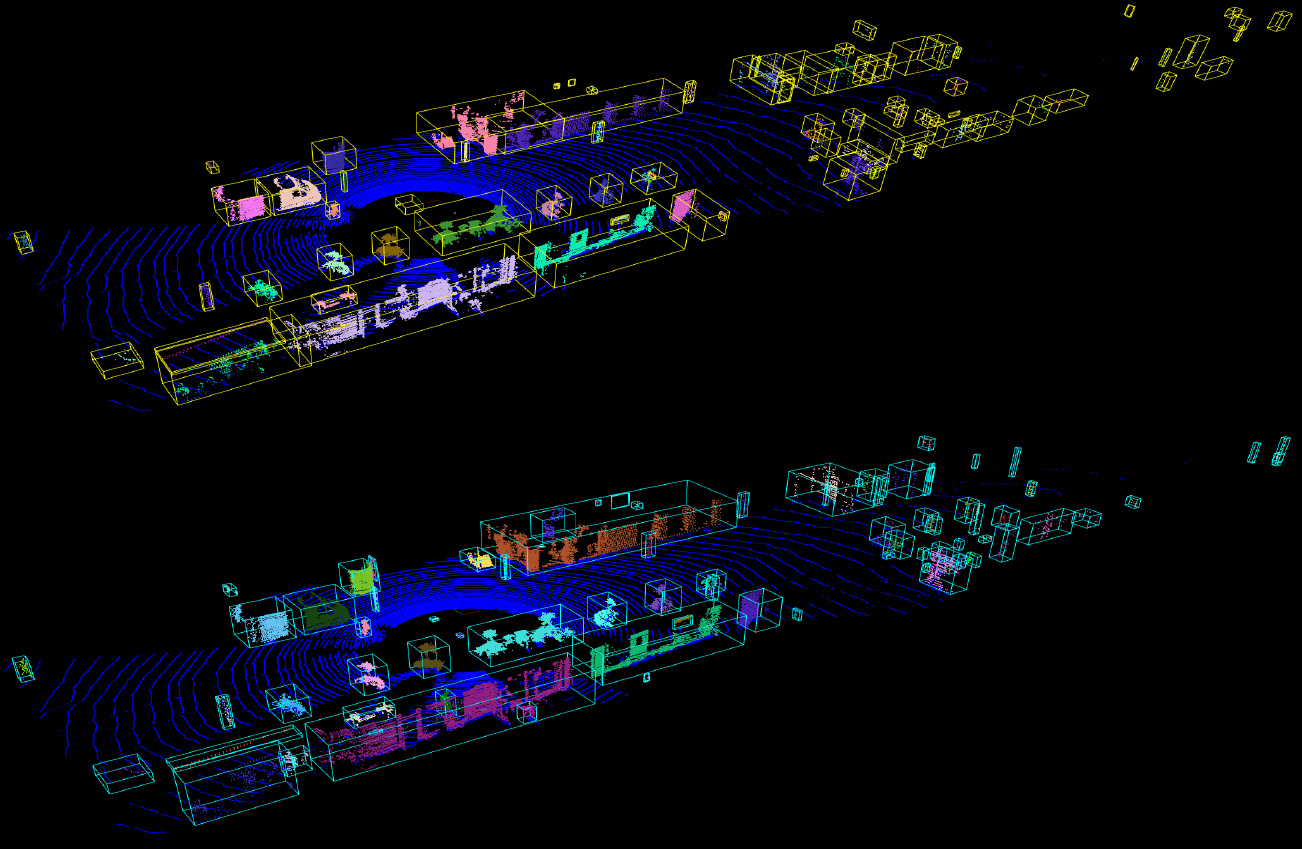
\includegraphics[width=15cm,height=7cm]{ClusteredPointCloud}
    \caption{Objektidentifizierung einer 3D-Punktwolke aus \cite{bib:Segmentation1}. Die Bodenpunkte der Wolke sind blau dargestellt und die Objekte sind mit Boxen gekennzeichnet.}
    \label{fig:ClusteredCloud}
\end{figure}

\subsubsection{Bodenpunkt-Analyse}
Wie schon erwähnt werden bei vielen Verfahren der Cluster-Analyse von Punktwolken zuerst die Bodenpunkte identifiziert. Dieses Verfahren wird auch in dieser Arbeit angewendet. Der Grund dafür ist, dass die Bodenpunkte nicht in das Suchverfahren nach Objektpunkten aufgenommen werden dürfen. Sie würden nicht nur die Suche nach echten Objektpunkten erschweren sondern auch das Ergebnis der Objektcluster verfälschen. Als Erklärung soll folgender, simpler Cluster-Algorithmus dienen:

\begin{enumerate}
\item Definiere einen Startpunkt.
\item Suche alle Punkte innerhalb von Radius \(x\). 
\item Führe 2. für jeden gefundenen Punkt aus bis keine Punkte mehr gefunden werden.
\end{enumerate} 

Alle Objekte die auf dem Boden stehen, also deren Punkte nahe an Bodenpunkten sind, würden mit dem obigen Algorithmus die Bodenpunkte mit in den Cluster aufnehmen. Dies kann sogar dazu führen, dass 2 Objekte, die mittels Bodenpunkten miteinander verbunden sind zu einem Cluster zusammengefügt werden. Die Segmentierung des Bodens wird in C.LABEL-VR nach dem Einlesen des internen Datenformates ausgeführt, also zwischen Import Addons und PCL Generator (siehe Abbildung \ref{fig:ImportExport}). Beim Erstellen der Punktwolken ist also schon bekannt welcher Punkt ein Bodenpunkt ist und welcher nicht. Dazu wird im internen Datenformat das Attribut für die Bodenpunktkennzeichnung mit dem entsprechenden Wert versehen. Wie diese Werte ermittelt werden ist im Folgenden erklärt.\\

Als Basis für die Bodenpunktanalyse in C.LABEL-VR wurde das \textit{Ground Plane Fitting}-Verfahren (GPF) aus \cite{bib:Segmentation1} verwendet. Ist im Folgenden die Rede von GPF, ist immer der Ansatz der eben zietierten Arbeit gemeint. Ziel dieses Verfahrens ist es ein mathematisches Modell einer Ebene zu errechnen, welches den Boden repräsentieren soll. Anschließend kann von jedem Punkt der Abstand zu dieser Ebene errechnet werden. Ist der Abstand eines Punktes kleiner als ein definierter Wert, so handelt es sich bei ihm um einen Bodenpunkt. Die Punktwolke, die analysiert werden soll, wird dabei zunächst in eine Anzahl an $N_{segs}$ Segmenten aufgeteilt. Der Algorithmus zur Identifizierung der Bodenpunkte wird für jedes dieser Segmente ausgeführt. Der Grund für diese Segmentierung ist die mögliche Unebenheit der Bodenfläche. Eine Ebene kann schließlich keine ungleichmäßige Fläche repräsentieren. Wird aber für jedes Segment der Punktwolke eine eigene Ebene ermittelt so verbessert sich das Ergebnis der Bodenpunktanalyse, wie in Abbildung \ref{fig:Segments} zu sehen ist.\\

\begin{figure}%
	\centering
    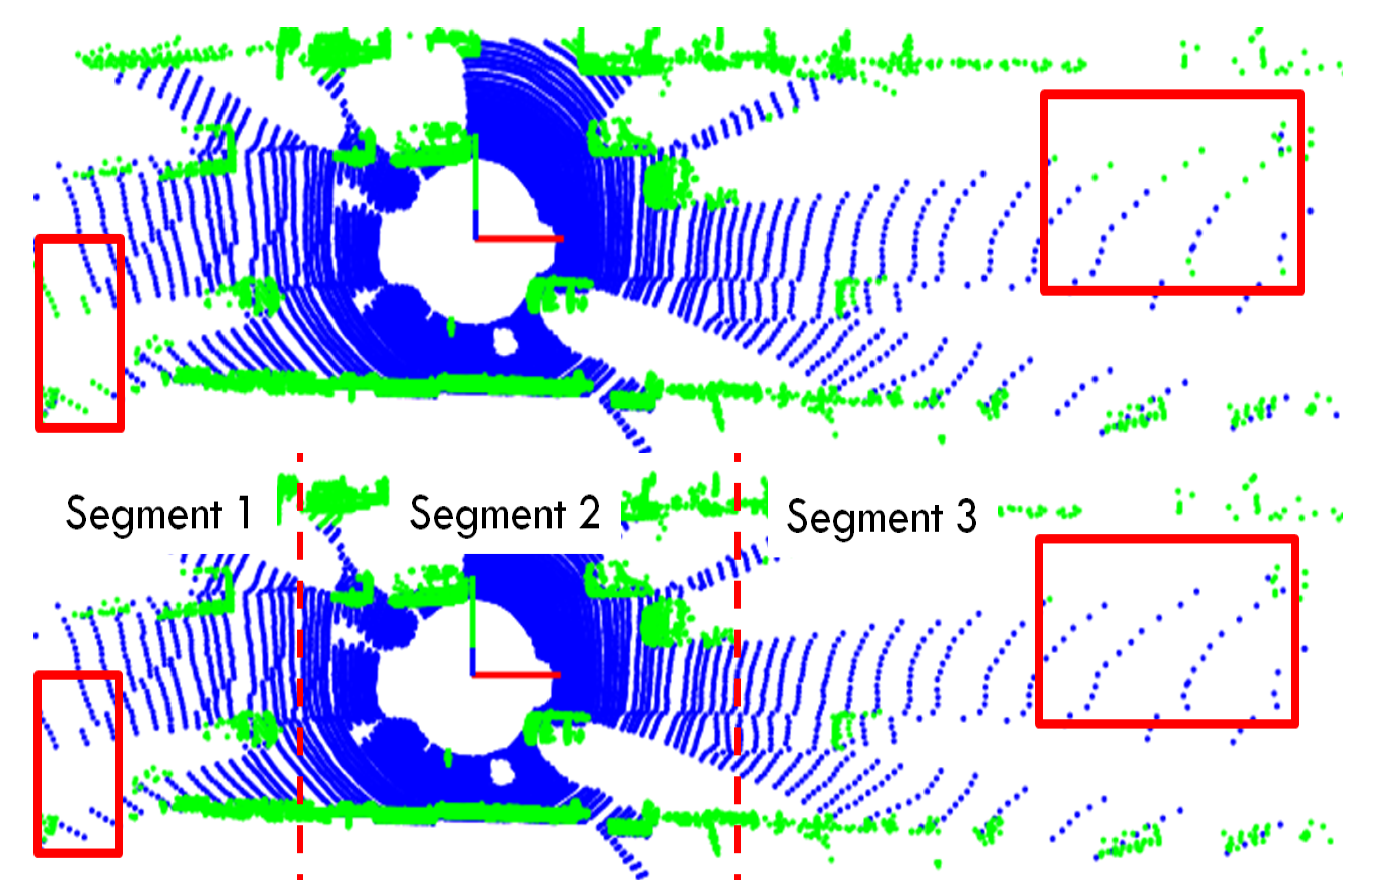
\includegraphics[width=12cm,height=7cm]{Segments}
    \caption{In \cite{bib:Segmentation1} wird gezeigt, dass die Segmentierung einer Punktwolke zu einem besseren Ergebnis der Bodenpunktanalyse führt. Die obere Abbildung ist dabei ohne Segmentierung und die untere mit Segmentierung. Bodenpunkte sind blau und Objektpunkte in grün dargestellt. Die roten Rechtecke kennzeichnen den Bereich in dem die Analyse schlechter bzw. besser ist.}
    \label{fig:Segments}
\end{figure}

Beim GPF-Verfahren in \cite{bib:Segmentation1} wurden Punktwolken in 3 große Segmente entlang der $x$-Achse eingeteilt, da diese Achse der Fahrtrichtung des Autos entspricht. Damit wurden für die Testdaten, die CMORE für diese Arbeit zur Verfügung stellte, keine zufriedenstellenden Ergebnisse erzielt (vgl. Abbildung \ref{fig:WrongSegments}). Das Problem ist, dass sich durch eine zu simple Segmentierung entweder zu viele oder zu wenige Bodenpunkte in einem Sektor befinden können. Bei zu vielen Bodenpunkten kann es sein, dass der Boden nicht linear verläuft. Auf der linken Seite des Autos könnte sich beispielsweise eine Anhöhe befinden und auf der rechten Seite ein flaches Gelände. In diese Unebenheit kann keine richtige Ebene eingesetzt werden.
!!!!!!BILDER!!!!!!!!!
Bei zu wenigen Bodenpunkten kann es sein, dass der Algorithmus die Ebene an Objekte annähert. Handelt es sich bei solchen Objekten beispielsweise um eine senkrechte Wand, könnten die vielen hohen Punkte die Ebene senkrecht werden lassen.\\

Darum wurde in dieser Arbeit ein Verfahren entwickelt, dass die Segmente nicht anhand ihrer Größe einteilt sondern nach der Anzahl der potentiellen Bodenpunkte, welche die Segmente enthalten. Potentielle Bodenpunkte sind diejenigen Punkte, welche sich in einem bestimmten Höhenbereich befinden. Der Höhenbereich wurde auf -0.5m bis 0.5m festgelegt. Das bedeutet alle Punkte, deren Höhenwert sich innerhalb des Wertebereichs befindet, sind potentielle Bodenpunkte. Das Segmentierungsverfahren erstellt nun die Segmente so, dass sich in jedem Segment gleich viele dieser potentiellen Bodenpunkte befinden. Zusätzlich zu der Segmentierung aus \cite{bib:Segmentation1} wurden die Segmente noch durch die $y$-Achse geteilt, um den vorher angesprochenen Problemfall der unterschiedlichen Geländebeschaffenheiten links bzw. rechts vom Auto auszugleichen. Das Ergebnis und der direkte Vergleich mit der normalen GPF-Methode ist in Abbildung \ref{fig:RightSegments} zu sehen. 

\begin{figure}[!tbp]
  \centering
  \begin{minipage}[b]{0.4\textwidth}
    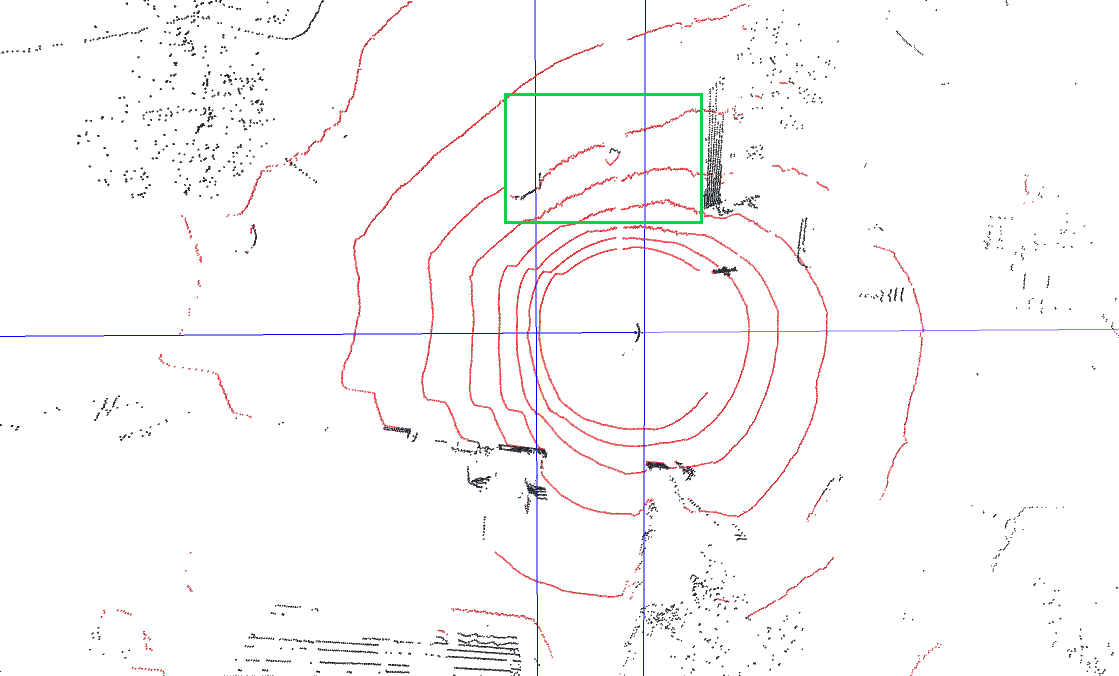
\includegraphics[width=\textwidth]{GroundSeg_BirdeyeWithSectors2}
    \tiny{\caption{Segmentierung anhand potentieller Bodenpunkten}}
    \label{fig:WrongSegments}
  \end{minipage}
  \hfill
  \begin{minipage}[b]{0.4\textwidth}
    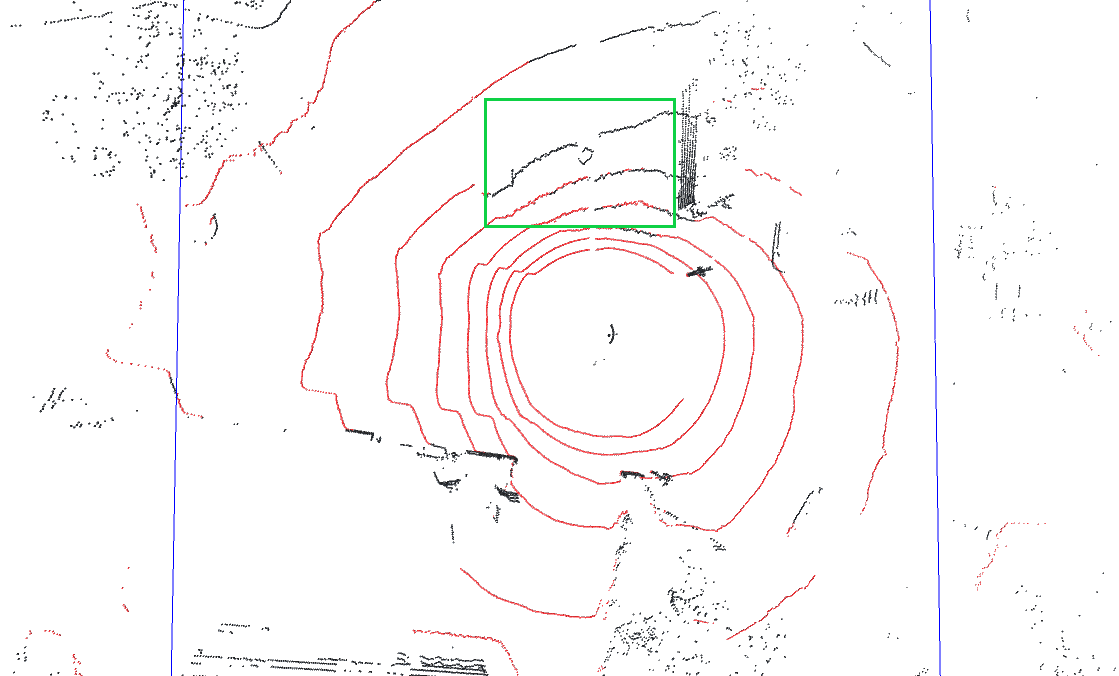
\includegraphics[width=\textwidth]{GroundSeg_BirdeyeWithWrongSectors2}
    \tiny{\caption{Segmentierung anhand Koordinaten entlang der $x$-Achse}}
    \label{fig:RightSegments}
  \end{minipage}
  
  \small{\caption {Vergleich der Segmentierungsmethoden zur Bodenpunktanalyse aus \cite{bib:Segmentation1} und C.LABEL-VR. Bodenpunkte sind rot, alle anderen schwarz. Die blauen Linien stellen die Trennung der Segmente dar. Die grünen Boxen markieren den Bereich, in dem man den Unterschied der beiden Methoden bei der Bodenpunkterkennung sieht.}}
    \label{fig:Segmentation}%
\end{figure}

\begin{algorithm}
  \caption{Algorithmus zur Einteilung einer Punktwolke in $N_{Segs}$ Segmente}
\label{alg:Segmentation}
  \begin{algorithmic}[1]
    \Inputs{\textbf{$\textbf{P}$} : Menge aller Punkte\\
    $N_{Segs}$} : Anzahl der Segmente}
    \Initialize{$\textbf{S}$ : Menge aller Segmente mit den jeweiligen Punkten
    $\textbf{P}_{pot}$} : Menge aller potentiellen Bodenpunkte\\
    $C_{segs} :$ Zähler des aktuellen Segments\\
    			$C_{points} :$ Zähler der Bodenpunkte des aktuellen Segments\\

   	\State \textbf{MainLoop:}
   	\State $\textbf{P} = \Call{SortAscendingByXValue}{\textbf{P}}$
  	\State $\textbf{P}_{pot} = \Call{GetPotentialGroundPointsBetween}{-0.5, 0.5, \textbf{|P|}} $;
  	\State $C_{segs} = C_{segs} = 0$;
    \For{$i=1 : |P|$}
      	\If{$p_i.yValue \geq 0$}
      		\State $\textbf{S}[C_{segs}] gets p_i$
      	\Else
      		\State $\textbf{S}[C_{segs}+1] gets p_i$
      	\EndIf
      	\If{$p_i.zValue \geq $}
      	\EndIf
      \EndFor

  \end{algorithmic}
\end{algorithm}












\begin{algorithm}
  \caption{Algorithmus zur Identifizierung von Bodenpunkten eines Punktwolken-Segments}
\label{alg:GroundPoints}
  \begin{algorithmic}[1]
    \Inputs{\textbf{$\textbf{P}$} : Menge aller Punkte der Wolke\\}
    \Initialize{\textbf{$\textbf{P}_{seeds}$} : Menge aller Seed-Punkte\\
    			%$N_{segs} :$ Anzahl der Segmente\\
    			$N_{iter} :$ Anzahl der Iterationen\\
    			$T_{init} :$ Distanzgrenzwert der initialen Seed-Punkte\\
    			$T_{plane} :$ Distanzgrenzwert zur geschätzten Ebene}
   	\State \textbf{MainLoop:}
  	\State $\textbf{P}_{seeds}$ = \Call{\textbf{GetInitialSeedPoints}}{$\textbf{P}$, $T_{init}$};
    \For{$i=1 : N_{iter}$}
      \State $plane$ = \Call{\textbf{FitPlaneIntoPoints}}{$\textbf{P}_{seeds}$};
      \State \Call{Clear}{$\textbf{P}_{seeds}$};
      \For{$j=1 : |\textbf{P}|$}
      	\State $distance$ = \Call{\textbf{GetDistanceToPlane}}{$plane$, $p_k$};
      	\If{$distance < T_{plane}$}
      		\State $p_k.groundpoint = true$;
      		\State $\textbf{P}_{seeds} \gets p_k$
      	\Else
      		\State $p_k.groundpoint = true$;
      	\EndIf
      \EndFor
    \EndFor
    \\
    \State \textbf{GetInitialSeedPoints:}
    \Initialize{\textbf{$\textbf{P}_{low}$} : Alle tiefen Punkte aus $\textbf{P}$\\
   			$H_{avg}$ : Durchschnittshöhe alle Punkte aus $\textbf{P}_{low}$}
    \For{$i=1 : |\textbf{P}|$}
    	\If{$p_i.height < 0.5 \And p_i.height > -0.5$}
    		\State $\textbf{P}_{low} \gets p_i$
    	\EndIf 
    \EndFor
    \State $H_{avg} = \Call{\textbf{GetAverageHeight}}{\textbf{P}_{low}}$;
    \For{$i=1 : |\textbf{P}|$}
    	\If{$p_i.height < T_{init}$}
    		\State $\textbf{P}_{seeds} \gets p:i$;
    	\EndIf 
    \EndFor
  \end{algorithmic}
\end{algorithm}




%https://en.wikipedia.org/wiki/Singular-value_decomposition
%https://www.ltu.se/cms_fs/1.51590!/svd-fitting.pdf
\subsubsection{Cluster-Analyse}


\section{User Interface}
\label{sec:UIMenu}
\subsection{Ingame Menu}
%\subsection{Movement}
%\subsection{Labelclasses}


